\newpage
%-------------------------------------------------------------------------
\subsection{Creep in salt rock}

Several models exists for the evaluation of the effect of stationary
creep in rock salt, i.e the strain variation with time is
calculated. One of those models is the BGRa-model
(\ref{eqn:BGRa_model}), which is valid for loads between 5 and 25
MPa in a temperature range of 22-200$^o$C (Hunsche and Schulze,
1994).
%
\begin{equation}
\dot\Stra^{c}
=
A e^{-\frac{Q}{R T}}
\left( \frac{\sigma}{\sigma^*} \right)^n
\label{eqn:BGRa_model}
\end{equation}
%
Table \ref{tab:creep_salt} depicts the symbols of equation
(\ref{eqn:BGRa_model}), their meaning and parameter values.
%
\begin{table}[H]
\center
\begin{tabular}{llrl}
\hline\noalign{\smallskip}
\hline
Symbol & Meaning & Value & Unit \\
\hline
$\dot\Stra$ & Strain rate & & 1/d \\
$\sigma$ & Effective stress & $$ & MPa \\
\hline
$A$ & Material constant & $0.18$ & 1/d \\
$Q$ & Activation energy & $54$ & kJ/mol \\
$R$ & Gas constant & $8.31447215$ & J/(K mol) \\
$n$ & Material constant & $5$ & -- \\
$\sigma^*$ & Reference effective stress & $1$ & MPa \\
\hline\hline
\end{tabular}
\caption{Creep model, symbols and material values} %\footnotesize
\label{tab:creep_salt}
\end{table}

\subsubsection*{Example 1: Temperature dropping (relaxation)}
\label{sec:creep_salt_example_1}

\paragraph*{Problem definition}
In a sample of rock salt a stress relaxation is caused by a
temperature decrease of 30 K. The aim of the example is to calculate
the resulting strain variation with time within the solid body by
the use of the stationary creep model BGRa (\ref{eqn:BGRa_model}).
The results of the simulation using an axial symmetric calculation
model and a 3D model are compared afterwards.

Assumptions
\begin{tabular}{|ll|}
\hline\noalign{\smallskip}
Heat  & Constant temperature in the whole body at the \\
      & beginning (330 K), temperature decrease of 30 K \\
Solid & Homogenous, finite dimensions, no deformation at the \\
      & boundaries in z-direction at the bottom and the top \\
\hline
\end{tabular}

\begin{figure}[H]
\centering
\includegraphics[scale=0.5]{M/creep_salt_1}
\caption{Core sample model}
\label{fig:creep_salt_1}
\end{figure}

For the 2D numerical simulation a cylindrical core sample as shown
in Fig. \ref{fig:creep_salt_1} is selected. The 2D numerical model
is an axial symmetric one in the x-z-plane (see Fig.
\ref{fig:creep_salt_2}). The dimensions of this 2D model are: 0.05 m
radius (x-direction) and 0.2 m of height. A relatively coarse mesh
consisting of 228 triangular elements and 139 nodes is used.
Vertical deformations at the top and the bottom are suppressed (no
displacement boundary conditions). The initial temperature in the
whole area is 330 K. At the top and the bottom of the model thermal
boundary conditions are set with a temperature of 300 K. Thereby the
stress relaxation during the cooling down is simulated. The used
parameters of the solid represent the material behavior of rock salt
are given in Tab. \ref{tab:creep_salt}. The calculation is divided
in 360 time steps with a constant time step length of 1 day.

\begin{figure}[H]
\centering
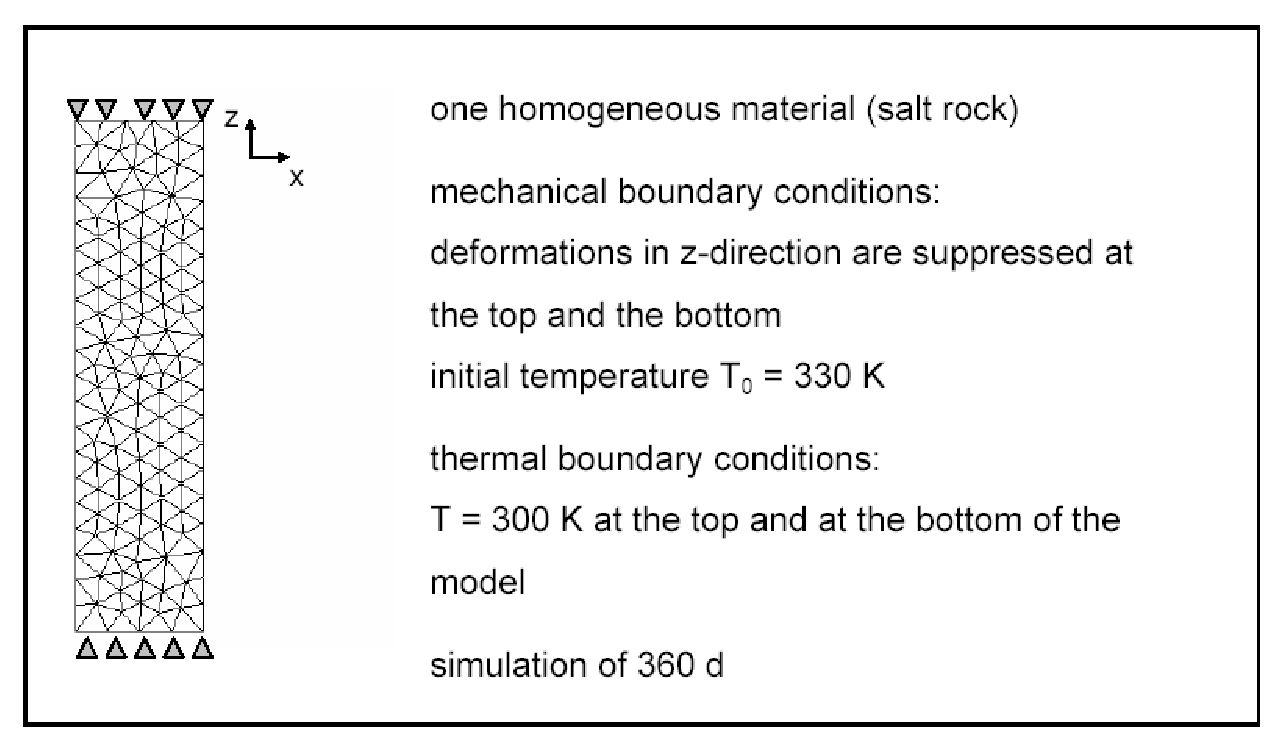
\includegraphics[scale=0.5]{M/creep_salt_2}
\caption{Numerical axisymmetrical model} \label{fig:creep_salt_2}
\end{figure}

Table \ref{tab:creep_salt_heat} depicts the values of material
properties for the thermo-mechanical creep model.
%
\begin{table}[H]
\center
\begin{tabular}{llrl}
\hline\noalign{\smallskip}
\hline
Symbol & Meaning & Value & Unit \\
\hline
$T_0$    & Initial temperature (before cooling down) & $330$ & K \\
$T$      & Temperature after cooling down & $300$ & K \\
$E$      & Young's modulus & $25$ & GPa \\
$\nu$    & Poisson ratio & $0.27$ & -- \\
$\alpha$ & Thermal expansion coefficient & $4\times 10^{-5}$ & 1/K \\
$c$      & Thermal capacity & $1$ & J/(kg K) \\
$\lambda$ & Thermal conductivity & $100$ & W/(m K) \\
\hline\hline
\end{tabular}
\caption{Material parameters of the thermo-mechanical creep model} %\footnotesize
\label{tab:creep_salt_heat}
\end{table}

\paragraph*{Analytical solution}
%
In order to evaluate the numerical results of the relaxation
problem, the analytical solution of equation
(\ref{eqn:BGRa_model_2}) (Eickemeier 2007, personal communication)
for the difference of effective stresses within one time step can be
applied.
%
\begin{equation}
\Delta\sigma_{i+1}
=
\frac
{(\dot\Stra^{c}_1 - A (\sigma/\sigma^*)^n) E_q \Delta t}
{1 - E_q / \sigma^* A^* \Delta t \xi n (\sigma/\sigma^*)^{n-1}}
\label{eqn:BGRa_model_2}
\end{equation}
%
and
%
\begin{equation}
A^*
=
A e^{-Q/RT}
\label{eqn:BGRa_model_3}
\end{equation}
%
where the initial strain rate $\dot\Stra^{c}_1$ in this case is
zero, $E_q$ in general is the weighted Young's modulus of the steel
plates and the salt rock sample (in this case we consider only salt
rock), $\xi$ = 0.5.

For the analytical solution of the equation (\ref{eqn:BGRa_model_2})
the vertical stress before the last time step is considered. Time
step increment is $\Delta t$ = 1 d. The calculation is done for node
705 of the 3D model (Fig. \ref{fig:creep_salt_3}), which is located
at point (x,y,z)=(0.05,0,0.12). The calculated stress difference
$\sigma_{i+1}$ has to be identical to the numerical result.

\begin{figure}[H]
\centering
\includegraphics[scale=0.28]{M/creep_salt_3}
\caption{Comparison of numerical results (GeoSys/RockFlow vs ANSALT) for vertical stresses}
\label{fig:creep_salt_3}
\end{figure}

\paragraph*{Results}
%
The comparison of the stress increment $\sigma_{i+1}$ which was
obtained by the use of equation (\ref{eqn:BGRa_model_2}) is
identical to the value (of vertical stresses) at node 705 (at the
same location as node 76, see Fig. \ref{fig:creep_salt_3}) of the 3D
numerical calculation. Both stress increments $\sigma_{i+1}$
obtained by GS/RF and ANSALT are equal to $3.05\times 10^{-3}$ MPa.
Additionally, the numerical results for vertical stresses of the 2D
simulation at node 76 are compared to the results that were obtained
by simulating the creep process by the FE programme ANSALT (Nipp
1988) and also to the results of the 3D simulation with GS/RF at
node 705. The comparison of the results of GS/RF in 2D and 3D with
the ANSALT findings are depicted in Fig. \ref{fig:creep_salt_3}.

The input data and boundary conditions for each calculation model
are identical. Also the results show a good accordance. That means,
the creep simulation (2D and 3D) of GS/RF by using the implemented
BGRa model provides correct results.

\subsubsection*{Benchmark deposit}

\begin{tabular}{|l|l|l|l|l|l|}
\hline
PCS type & MSH type       & Files   & Version    & Date    & Author\\
\hline
TM       & axial-symmetry & BGRa    & 4.4.10(WW) & 13.03.07 & BGR \\
\hline
TM       & axial-symmetry & creep3d & 4.4.10(WW) & 13.03.07 & BGR \\
\hline
\end{tabular}

%-------------------------------------------------------------------------
\subsubsection*{Example 2: Creep under constant load}

\paragraph*{Problem definition}
%
In the same example that is described in section
\ref{sec:creep_salt_example_1} the creep process is now assumed to
be caused by a constant load at the bottom of the solid and a
constantly high temperature at the same time. The aim of this
example is to calculate the resulting strain variation with time by
using the stationary creep model BGRa (\ref{eqn:BGRa_model}).

We specify the initial and boundary conditions for the 2D numerical
model. For the simulation with GS/RF almost the same calculation
models (2D and 3D) as in the precedent creep example were selected.
Only the height of the solid is 0.25 m instead of 0.2 m. The initial
temperature in the whole area is 373.15 K. There is a constant load
of 5 MPa at the bottom of the model as boundary condition. The
calculation is divided in 100 time steps with a constant time step
length of 1 day.

\paragraph*{Analytical solution}
%
In order to find out, whether the numerical solutions of
GeoSys/RockFlow accord to the results of the BGRa model
(\ref{eqn:BGRa_model}), the input parameter $A$ is compared to the
$A$, which results from the simulation run. For this calculation
equation (\ref{eqn:BGRa_model}) is converted to the following
expression.
%
\begin{equation}
A
=
\frac
{\dot\Stra^{c}}
{e^{-Q/RT} \sigma_{\mbox{\footnotesize eff}}}
\label{eqn:BGRa_model_4}
\end{equation}
%
with
%
\begin{eqnarray}
\sigma_{\mbox{\footnotesize eff}}
&=&
\frac{1}{\sqrt{2}}
\sqrt{(\sigma_1-\sigma_2)^2 + (\sigma_2-\sigma_3)^2 + (\sigma_3-\sigma_1)^2}
\nonumber
\\
\dot\Stra
&=&
\frac
{\Stra_{\mbox{\footnotesize eff}}(t+\Delta t) - \Stra_{\mbox{\footnotesize eff}(t)}}
{\Delta t}
\\
\Stra_{\mbox{\footnotesize eff}}
&=&
\frac{\sqrt{2}}{3}
\sqrt{(\Stra_1-\Stra_2)^2 + (\Stra_2-\Stra_3)^2 + (\Stra_3-\Stra_1)^2}
\nonumber
\label{eqn:BGRa_model_5}
\end{eqnarray}

For these calculation steps the stresses of the regarded time period
have to be constant. Equations (\ref{eqn:BGRa_model_5}) are solved
for node 25 (see Fig. \ref{fig:creep_salt_4}) of the 2D numerical
model. The last time step at $t$ = 100 days of the simulation run
was considered.
%
\begin{figure}[H]
\centering
\includegraphics[scale=0.26]{M/creep_salt_4}
\caption{Comparison of 2D and 3D numerical results for strains (x- and z-directions)}
\label{fig:creep_salt_4}
\end{figure}
%
\begin{figure}[H]
\centering
\includegraphics[scale=0.37]{M/creep_salt_5}
\caption{Comparison of 2D and 3D numerical results for strains (y-direction)}
\label{fig:creep_salt_5}
\end{figure}

\paragraph*{Results}
%
The effective stress $\sigma_{\mbox{\footnotesize eff}}$ at node 25
and for the given time span is 5.03 MPa, which was calculated by the
use of equation (\ref{eqn:BGRa_model_5}). The strain of time step 1
is $\Stra_{\mbox{\footnotesize eff}}(t_1)$ = $1.72\times 10^{-3}$
and of time step 2: $\Stra_{\mbox{\footnotesize eff}}(t_2)$ =
$1.73\times 10^{-3}$ , calculated by equation
(\ref{eqn:BGRa_model_5}), is equal to $1.6 \times 10^{-5} d^{-1}$.
After equation (\ref{eqn:BGRa_model_4}) the calculated parameter $A$
is equal to 0.19, which corresponds approximately to the input $A$
of 0.18. Therefore, it can be summarized that the BGRa creep model
is implemented in GeoSys/RockFlow properly. The comparison between
the 2D (node 25) and 3D results (node 705) are depicted in Fig.
\ref{fig:creep_salt_4} and Fig. \ref{fig:creep_salt_5}. The 2D and
3D results are identical to each other.

\subsubsection*{Benchmark deposit}

\begin{tabular}{|l|l|l|l|l|l|}
\hline
PCS type & MSH type       & Files     & Version    & Date    & Author\\
\hline
M       & axial-symmetry & uc\_creep01 & 4.4.10(WW) & 13.03.07 & BGR \\
\hline
M       & axial-symmetry & uc\_creep3d & 4.4.10(WW) & 13.03.07 & BGR \\
\hline
\end{tabular}
